% !TEX root = master.tex
\chapter{Projektsteckbrief}
\section{Grundlagen}
\label{chapter:1}

\begin{center}
	\begin{tabularx}{\textwidth}{|l|X|}
		\hline
		\textbf{Projektname} & Digipaper \\
		\hline
		\textbf{Auftraggeber} & Geschäftsführung des Unternehmens CP Service GmbH \\
		\hline
		\textbf{Tragweite} & Deutschlandweit \\
		\hline
		\textbf{Dauer} & 12 Monate \\
		\hline
		\textbf{Phasen} 
		& 1 Monat: Konzeptionelle Arbeit \\
		& 4 Monate: Entwicklung \\
		& 1 Monat: Testing \\
		& 3 Monate: Pilotierung bei den Großkunden \\
		& 3 Monate: Allgemeiner Rollout \\
		\hline
		\textbf{Zieltermin} & 12 Monate nach dem Start \\
		\hline
	\end{tabularx}
\end{center}
\captionof{table}{Kopfdaten für das Projekt der CP Service GmbH} \label{tab:kopfdaten}\vspace{10pt}

Die CP Service GmbH ist ein Unternehmen mit internationalen Standorten, ungefähr 1.200 Mitarbeitern und Firmensitz in Mannheim. Das Kerngeschäft liegt im Auftreten als Mittler zwischen Handelsketten und Kreditinstituten, um Zahlungen verarbeiten zu können. Auftragseingänge von Kunden, welche das Anmelden, Aktualisieren und Löschen von Filialen betreffen, können aktuell nur in Papierform an die CP Service GmbH gesendet werden. Hierdurch entstehen hohe Aufwände und Verzögerungen, worunter die Mitarbeiter- und Kundenzufriedenheit leiden. Abseits von Verzögerungen durch den Postverkehr sind auch die Verarbeitungsprozesse von einer erheblichen Ineffizienz geprägt, da die Mitarbeiter diese handgeschrieben Aufträge entziffern müssen und es oft zu fehlerhaften Angaben kommt. Die mangelnde digitale Transformation hat bereits zwei unverzichtbare Großkunden dazu veranlasst mit der Kündigung zu drohen, weshalb dringender Handlungsbedarf besteht. Den Großkunden wurde bereits mehrfach die Digitalisierung der Schnittstellen zugesichert, allerdings kam es aufgrund mangelnder Kapazitäten nie zur Umsetzung. Da die CP Service GmbH sich aktuell in einer wirtschaftlich herausfordernden Situation befindet, würde der Verlust dieser Großkunden die Solvenz des Unternehmens erheblich beeinträchtigen. Daher hat die Geschäftsführung ein starkes Interesse an der zeitnahen Digitalisierung von den Schnittstellen.
Dies soll mithilfe eines neuen Projektes bewältigt werden, sodass die Großkunden befriedigt und die Zukunft des Unternehmens gesichert werden kann. Die Tabelle \ref{tab:kopfdaten} stellt die Kopfdaten des Projekts \textit{"Digipaper"} dar. 
\vspace{10pt}

Das Projektziel umfasst die Digitalisierung der Schnittstellen für das Anlegen, Ändern und Löschen von Filialen, sodass eine Steigerung der Effizient und eine Verbesserung der Kunden- und Mitarbeiterzufriedenheit erzielt werden kann. Das Projekt soll vorerst lediglich in Deutschland umgesetzt werden, obwohl CP Service GmbH über eine internationale Kundenbasis verfügt. Neben der vereinfachten Verarbeitung von Aufträgen steht insbesondere auch die Ermöglichung von Rückfragen im Fokus, um die Kommunikation zwischen den Sachbearbeitern der beteiligten Unternehmen zu fördern. Des Weiteres soll es den Kunden ermöglicht werden, Auswertungen über das getätigte Gesamtvolumen an Zahlungseinnahmen pro Handelsfiliale über eine weitere Schnittstelle einzusehen. All das soll die Servicequalität verbessern und die Großkunden langfristig an das Unternehmen binden. Hierzu ist ein Softwareprodukt zu entwickeln, welches einen digitalen Informationsaustausch zwischen der CP Service GmbH und dessen Kunden ermöglicht. 


\section{Projektinhalt und Abgrenzung}
Das Projekt beinhaltet die Digitalisierung von drei spezifischen Formularen, die momentan noch per Post versendet und von Sachbearbeitern verarbeitet werden. Das erste Formular betrifft das Anbinden neuer Filialen, womit es ihnen ermöglicht wird neue Kartenzahlungen abzuwickeln. 
Ein zweites Formular wird genutzt, um Änderungen der Kontaktdaten einer Filiale zu übermitteln. Das dritte Formular dient der Löschung von Filialen, welche geschlossen oder abgerissen wurden. 
Zusätzlich zu diesen Formularen wird eine Software eingeführt, welche die Bearbeitung und Archivierung der Aufträge ermöglicht. Ein weiterer Bestandteil des Projekts ist die Einrichtung eines digitalen Kommunikationskanals, der Rückfragen der Sachbearbeiter erleichtert. Auch die regelmäßig an Kunden versendeten Auswertungen über das getätigte Gesamtvolumen an Zahlungseinnahmen pro Handelsfiliale wird durch das Projekt digitalisiert. 
Der Rollout des Projekts wird sich auf Deutschland beschränken. Es wird eine Webapplikation entwickelt werden, welche eigene Mitarbeiter und Kunden für die Kommunikation und den Informationsaustausch verwenden können. Innerhalb dieser Applikation gibt es nach einem initialen Anmeldevorgang unterschiedliche Masken für Sachbearbeiter und Kunden. Während die Kunden neue Aufträge anlegen und versenden können, sind die Sachbearbeiter in der Lage mit diesen anschließend zu arbeiten. Die Webapplikation basiert auf mehreren XML-Schnittstellen, welche den kommunikativen Austausch ermöglichen werden.

\begin{figure}[h!]
	\centering 
	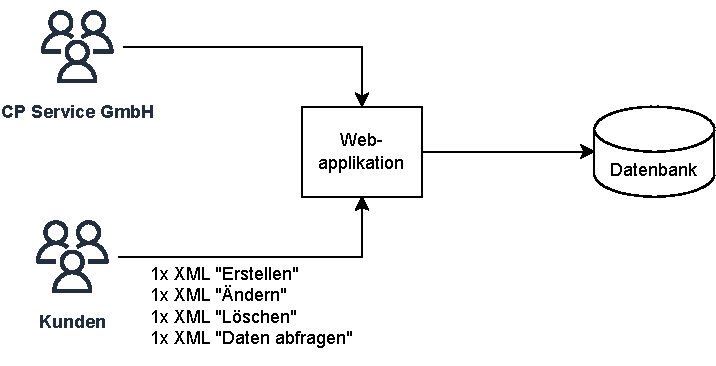
\includegraphics[scale=1]{img/konzept.pdf}
	\captionsetup{format=hang}
	\caption[Projektinhalt Skizze]{\label{fig:konzept} Konzeptioneller Aufbau des technischen Projektinhalts}
\end{figure}

Abbildung \ref{fig:konzept} zeigt den technischen Aufbau des Projektes. Zentraler Bestandteil ist eine Webapplikation, welche von den Kunden oder Sachbearbeitern der CP Service GmbH mithilfe von XML Schnittstellen verwendet werden kann. Diese Applikation kommuniziert mit einer Datenbank, in welcher relevante Daten persistent gespeichert werden.
Nicht Teil des Projektes ist zudem die Digitalisierung der unterschiedlichen Zahlungsaktivitäten von den Kunden unserer Kunden innerhalb der Handelsfilialen.

\clearpage
\section{Risiken und Nutzen}
\textbf{Risiken bei Durchführung}
\vspace{0.1cm}

Trotz sorgfältiger Planung und Vorbereitung ist die Durchführung des Projekts mit diversen Risiken verbunden. Ein zentrales Risiko des Projektes liegt in der Vernachlässigung von Kunden- oder Mitarbeiteranforderungen. Da dem Projekt eine hohe zeitliche Dringlichkeit zugrunde liegt ist es möglich, dass Anforderungen nicht ausreichend berücksichtigt werden. Bei ausbleibender Implementierung dessen kann es zu Frust und Ablehnung der Kunden und Mitarbeiter kommen, sodass das entwickelte Softwareprodukt nicht verwendet wird. Dies wäre fatal, da die Großkunden bereits sehr unzufrieden mit dem derzeit angebotenen Service sind und auch eine hohe Grundverstimmung innerhalb der eigenen Belegschaft besteht. Ein weiteres Risiko birgt die Zusammenstellung des Projektteams. Es ist von zentraler Bedeutung, dass das Team aus erfahrenen und kompetenten Mitarbeitern besteht, welche in der Lage sind in kurzer Zeit gute Ergebnisse zu liefern. Allerdings hat jeder interne oder externe Mitarbeiter individuelle Ansichten und Arbeitsweisen. Dies kann erheblichen Konflikten und Auseinandersetzungen führen, welche die Produktivität des Teams abseits der \textit{Storming} Phase von Tuckman negativ beeinflusst. Zu hohe Konfliktpotentiale können daher die Konsequenz einer Überschreitung zeitlicher Ressourcen haben, sodass das zu entwickelnde Softwareprodukt nicht rechtzeitig an die Kunden geliefert werden kann oder eine zu geringe Qualität aufweist. Es ist von zentraler Bedeutung Risiken wie diese frühzeitig zu erkennen und präventive Gegenmaßnahmen zu konzipieren. Das Kapitel \ref{chapt:Risikomanagement} widmet sich daher dem Risikomanagement und geht auf sämtliche Risiken und deren Gegenmaßnahmen im Detail ein.
\vspace{10pt}

\textbf{Risiken bei Nichtdurchführung}
\vspace{0.1cm}

Bei der Nichtdurchführung des Projektes entsteht zusätzlich das Risiko, dass Großkunden kündigen. Diese haben bereits in der Vergangenheit mit Kündigung gedroht, konnten aber durch das Versprechen von Verbesserungsmaßnahmen zum Verbleib bewogen werden. Da die Geschäftsführung dieses Versprechen allerdings über mehrere Jahre nicht einhalten konnte, sind die Großkunden gegenüber der CP Service GmbH negativ gestimmt. Im Falle der Nichtdurchführung ist es äußerst wahrscheinlich, dass diese Großkunden nicht mehr die Leistungen der CP Service GmbH beziehen. Dies wäre ein fataler Schlag für das Unternehmen, da die Solvenz von diesen Großkunden abhängig ist. Selbst wenn die CP Service GmbH in der Lage wäre das Abspringen dieser Kunden zu überleben, ist der Verlust weiterer Kunden nicht ausschließbar. Die Umsetzung des Projekts ist daher von höchster Priorität, um die CP Service GmbH zu retten. 

\vspace{10pt}
\textbf{Qualitativer Nutzen}
\vspace{0.1cm}

Der qualitative Nutzen des Projekts ist umfangreich und vielfältig. Durch die Digitalisierung der Auftragseingänge und die Implementierung der neuen Software, können Bearbeitungsprozesse optimiert und effizienter gestaltet werden. Dies führt nicht nur zur Aufwandsminimierung im Posteingang und der -aufbewahrung, sondern eliminiert auch die Notwendigkeit der manuellen Kontrolle und Entzifferung von Freitextfeldern. 
Die resultierende Effizienzsteigerung trägt zur gesteigerten Zufriedenheit der Mitarbeiter bei, insbesondere der Sachbearbeiter, und verbessert die Skalierbarkeit des Geschäftsmodells. Durch schnellere Bearbeitungszeiten und verbesserte Kommunikationswege wird die Zufriedenheit und Loyalität der Kunden erhöht. Es ist auch zu erwarten, dass positive Mund-zu-Mund-Propaganda das Image des Unternehmens stärkt und es sich positiv vom Wettbewerb abheben kann. Ein weiterer bedeutender Nutzen liegt in der Erfüllung der gegenüber den Großkunden gemachten Versprechen. Durch die Umsetzung des Projekts können Schäden der eigenen Reputation abgewendet und Vertrauen aufgebaut werden. Dies führt voraussichtlich dazu, dass die Großkunden erhalten bleiben und somit der langfristige Erfolg der CP Serivce GmbH gesichert wird.

\vspace{10pt}
\textbf{Quantitativer Nutzen}
\vspace{0.1cm}

Die Digitalisierung der Auftragseingänge hat das Potenzial, ebenfalls einen signifikanten quantitativen Nutzen zu generieren. Erwartet wird eine Vermeidung des Umsatzeinbruchs durch den Erhalt der zwei Großkunden. Die erhöhte Effizienz und Kundenorientierung kann zudem neue Kunden anziehen. Im internen Bereich kann durch eine Reduktion des Personals in der Poststelle und die Freigabe von Lagerfläche eine Kostenreduktion erzielt werden. Durch eine beschleunigte Inbetriebnahme von Zahlungsgeräten in den Filialen wird zudem die Provision gesteigert. Auch fallen durch den Verzicht auf Postversand weitere Kostenersparnisse an. Erfolgsfaktoren für diese Ertragssteigerung sind ein passendes Lösungsdesign, gründliches Testing, eine gut geplante Pilotierungsphase, ausreichende Ressourcen, klare Kundenkommunikation und solides Domänenwissen.

\section{Rahmenbedingungen und Annahmen}

\textbf{Voraussetzungen, Rahmenbedingungen \& Abhängigkeiten}
\vspace{0.1cm}

Es gibt diverse Voraussetzungen und Rahmenbedingungen für das Projekt \textit{Digipaper}. Zu Beginn muss ein Lösungsdesign für die digitalen XML Schnittstellen vereinbart werden. Alle Kunden müssen in der Lage sein, die relevanten Anfragen mit anschließend digital zu übermitteln, sodass die papierbasierte Kommunikation obsolet wird. Gleichzeitig müssen allerdings auch in der CP Service GmbH ausreichend Ressourcen für die Umsetzung des Projekts verfügbar und geeignete Mitarbeiter mit entsprechendem Fachwissen vorhanden sein. Zudem muss das Unternehmen sicherstellen können, dass eine gründliche Testphase durchgeführt wird, um Fehler präventiv vorzubeugen und einen komplikationslosen Produktivbetrieb zu gewährleisten. Des Weiteren werden zusätzlich einige Annahmen getroffen, um die Planung des Projekts durchführen zu können. So wird davon ausgegangen, dass beide Großkunden mit der digitalen Umstellung des Auftragseingangs befriedigt werden und von deren angedrohten Kündigung absehen. Zudem wird angenommen, dass die entwickelten Schnittstellen den Informationsfluss verbessern und Rückfragen erleichtern. Dies ist insbesondere zum Start des Rollouts vermutlich noch nicht vollständig gegeben, da Anwender Einarbeitungszeit benötigen. 

\vspace{10pt}
\textbf{Grobe Annahmen der Projektkosten}
\vspace{0.1cm}

Die Kosten für das Projekt können in mehrere Hauptkategorien eingeteilt werden. Personalkosten sind der größte Posten, sie umfassen Gehälter für das Projektteam, das aus Entwicklern, Testern, Projektmanagern und Supportpersonal besteht. Die Größe und Zusammensetzung des Teams hängt von den spezifischen Anforderungen des Projekts ab, wir können jedoch eine Teamgröße von 10 Vollzeitstellen für die Dauer von 12 Monaten annehmen.
Neben den Personalkosten fallen laufende Kosten für Software, Hardware und Infrastruktur an. Dazu gehören Lizenzen für Entwicklungs- und Testwerkzeuge, Serverkosten und Wartungsverträge. Je nach den spezifischen Anforderungen des Projekts können auch Kosten für die Anschaffung neuer Hardware oder die Aktualisierung bestehender Systeme anfallen.
Die Kosten für Umschulungen und Weiterbildungen sind ein weiterer wesentlicher Bestandteil. Sie decken Schulungen und Materialien hierfür ab, welche benötigt werden um die Mitarbeiter mit den neuen digitalen Systemen und Prozessen vertraut zu machen.
Zudem sind Kosten für Vermarktung und Kundenkommunikation zu berücksichtigen. Diese umfassen die Erstellung und Verbreitung von Marketingmaterialien und Kundeninformationen, sowie eventuell die Anpassung der Unternehmenswebsite oder der Kundenschnittstellen.
Insgesamt sollten diese Kostenpositionen ein umfassendes Bild der erwarteten Projektkosten liefern, wobei immer auch unvorhergesehene Kosten berücksichtigt werden sollten. Tabelle \ref{tab:anname_kosten} zeigt grobe Annahmen über die Höhe der Projektkosten. Es ist zu beachten, dass es sich hierbei nicht um die finalen Gesamtkosten, sondern lediglich um eine erste Schätzung, handelt.

\begin{table}[h!]
	\centering
	\begin{tabular}{|p{3cm}|p{8.3cm}|p{2cm}|} 
		\hline
		\textbf{Kostenkategorie} & \textbf{Beschreibung} & \textbf{Annahme}\\ [0.5ex] 
		\hline
		Personalkosten & Projektteam bestehend vermutlich aus circa 6 Vollzeitstellen. Durchschnittliche Vergütung inklusive sozialer Abgaben von 60.000€/Jahr. Es ist eine Projektlaufzeit von 12 Monaten angesetzt. & 360.000€ \\ 
		\hline
		Softwarekosten & Für die Entwicklung und den Betrieb wird externe Software verwendet. Es werden 5.000€ Lizenzkosten pro Teammitglied und 10.000€ anderweitige Softwarekosten angenommen. & 15.000€ \\ 
		\hline
		Kommunikation \& Vermarktung & Es ist professionelles Marketingmaterial zu erstellen, um Akzeptanz und Verständnis für die neue Lösung zu fördern. & 10.000€ \\ 
		\hline
		\textbf{Gesamtkosten} & & \textbf{385.000€} \\ 
		\hline
	\end{tabular}
	\caption{Grobe Annahmen der Projektkosten}
	\label{tab:anname_kosten}
\end{table}


